\subsection*{Část A}

\subsubsection*{Graf s jednotlivými kroky}
Tento subplot vykresluje napřed původní mapu, poté mapu převedenou do YCbCr s tím, že byla využita pouze složka Y, na níž byl dále aplikován Gaussův pohyblivý filtr (kernel). Dále jsou vykresleny hodnoty korelací a nakonec jsou v původní mapě červenými obdélníky vykresleny nalezené vesnice s kostelem.

\begin{figure}[H]
    \centering
    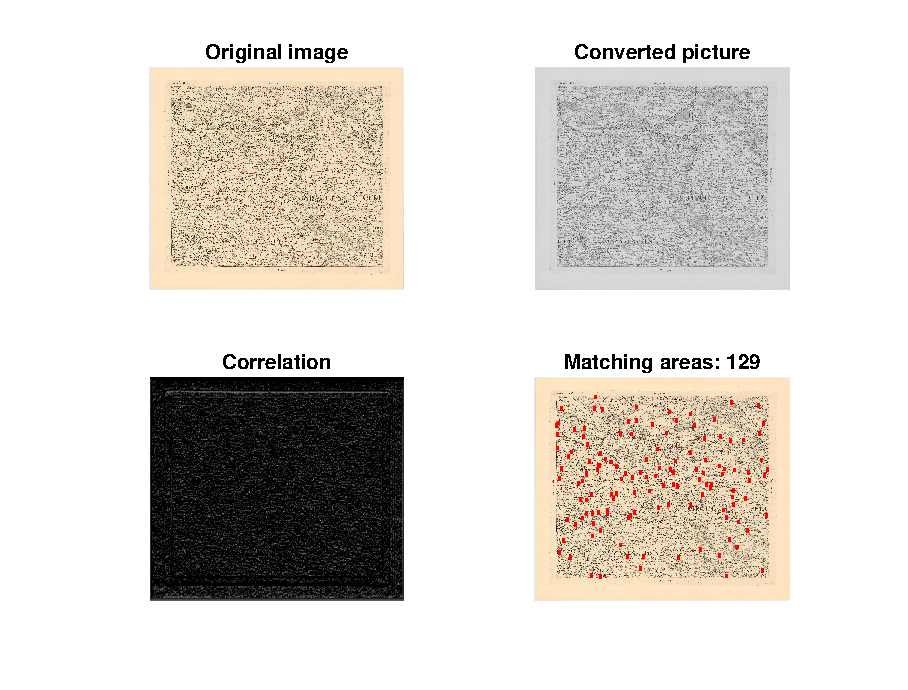
\includegraphics[width=0.8\textwidth]{images/plots.eps}
    \caption{Původní obrázek, konvertovaný obrázek s využitím složky Y prostoru YCBCR a následnou aplikací Gaussova filtru, hodnoty korelací a nalezené obce s kostelem označené červenými obdélníky}
\end{figure}

\subsubsection*{Detail nalezených obcí s kostelem}
\begin{figure}[H]
    \centering
    \includegraphics[width=0.8\textwidth]{images/found_villages.eps}
    \caption{Detail nalezených vesnic}
\end{figure}

\subsubsection*{Souřadnic nalezených bodů}
\begin{table}[H]
    \centering
    \textit{Tabulka 1: Souřadnice nalezených vesnic s kostelem}
    
    \begin{tabular}{|c c||c c||c c|}
    \hline
    \textbf{X} & \textbf{Y} & \textbf{X} & \textbf{Y} & \textbf{X} & \textbf{Y} \\
    \hline
    5499 & 3335 & 4373 & 1029 & 1601 & 1243 \\ \hline
    3289 & 5291 & 1727 & 6910 & 1826 & 5698 \\ \hline
    3131 & 5067 & 4441 & 6253 & 4180 & 1782 \\ \hline
    3753 & 1409 & 2308 & 4776 & 5532 & 1122 \\ \hline
    1071 & 4135 & 2069 & 1622 & 2840 & 4171 \\ \hline
    1931 & 6403 & 4085 & 2252 & 2173 & 726 \\ \hline
    914 & 3120 & 2536 & 3440 & 971 & 832 \\ \hline
    1486 & 4908 & 2918 & 4278 & 863 & 6869 \\ \hline
    5211 & 6215 & 3912 & 4112 & 3085 & 3004 \\ \hline
    4253 & 7123 & 1826 & 1507 & 1364 & 2880 \\ \hline
    3033 & 3712 & 2543 & 6955 & 3108 & 780 \\ \hline
    1323 & 4375 & 5016 & 896 & 2509 & 2176 \\ \hline
    1342 & 3144 & 2716 & 1985 & 2825 & 4985 \\ \hline
    2808 & 840 & 5510 & 2851 & 2545 & 5250 \\ \hline
    6089 & 1752 & 5150 & 2650 & 1479 & 697 \\ \hline
    2203 & 3777 & 3603 & 5159 & 4076 & 5812 \\ \hline
    3124 & 2667 & 3385 & 5400 & 2588 & 1705 \\ \hline
    4322 & 1479 & 3186 & 1487 & 2818 & 5845 \\ \hline
    4703 & 2039 & 4186 & 1613 & 2963 & 2793 \\ \hline
    3316 & 3963 & 3768 & 1613 & 3603 & 1760 \\ \hline
    1574 & 1527 & 3257 & 1345 & 5871 & 3271 \\ \hline
    4869 & 1771 & 3712 & 2425 & 4189 & 2241 \\ \hline
    3478 & 6118 & 2852 & 6151 & 2916 & 3264 \\ \hline
    1412 & 734 & 1757 & 698 & 4518 & 1278 \\ \hline
    3025 & 7070 & 2791 & 3841 & 5473 & 5685 \\ \hline
    2346 & 2046 & 1740 & 2655 & 4302 & 2897 \\ \hline
    3298 & 5419 & 2730 & 5679 & 1295 & 5524 \\ \hline
    2437 & 1062 & 3283 & 4256 & 3354 & 4379 \\ \hline
    2293 & 1151 & 3581 & 2382 & 4311 & 5885 \\ \hline
    3731 & 6478 & 4984 & 5982 & 1443 & 3623 \\ \hline
    6097 & 5883 & 5524 & 4410 & 4497 & 1808 \\ \hline
    2931 & 6570 & 5939 & 6982 & 3066 & 3427 \\ \hline
    3926 & 4786 & 3169 & 6600 & 5376 & 768 \\ \hline
    2942 & 5198 & 3896 & 6113 & 6115 & 2017 \\ \hline
    1128 & 4799 & 4161 & 3059 & 3488 & 3521 \\ \hline
    3561 & 2533 & 2575 & 4337 & 974 & 1858 \\ \hline
    3532 & 3070 & 773 & 6056 & 4144 & 1982 \\ \hline
    2831 & 7163 & 1417 & 7042 & 4237 & 2957 \\ \hline
    5278 & 5097 & 3680 & 6074 & 993 & 2078 \\ \hline
    2736 & 2520 & 1935 & 6024 & 2599 & 2353 \\ \hline
    1878 & 5206 & 2823 & 1943 & 1711 & 4060 \\ \hline
    609 & 1886 & 2949 & 1613 & 4712 & 6523 \\ \hline
    2971 & 5783 & 4017 & 3798 & 1749 & 2976 \\ \hline
    \end{tabular}
\end{table}
\newpage


